% Chapter Template

\chapter{Related Work} % Main chapter title

\label{Chapter2} % Change X to a consecutive number; for referencing this chapter elsewhere, use \ref{ChapterX}

%General explanation: We have an escape room that is currently a WSN with only little data processing, we watn to extend the middleware
% to achieve a broader spectrum of integration possibilities.
As explained in Chapter \ref{Chapter1}, the goal of this project was to extend an existing project.
Therefore, possible architectures and practices to integrate to the project were investigated.
In the following, research concerning the development of our project is listed and explained.

\section{Design Thinking}
Design thinking is one strategy to design a product or an innovation process.
As an innovation process, Plattner, Meinel and Leifer describe this process as "re-defining the problem, needfinding and benchmarking, ideating, building, testing." \parencite{designThinkingBook}
It seemed to fit the project and was a guide concerning the production phase, further explained in Chapter\ref{Chapter4}.
In contrast to mechanical improvements, design thinking tries to emphatize with possible customer needs at all parts of the product.
A few of design thinking's key principles are to 
"engage in early exploration of selected ideas, rapidly modelling potential solutions to encourage learning 
while doing, and allow for gaining additional insight into the viability of 
solutions before too much time or money has been spent" and that it 
"Iterates through the various stages, revisiting empathetic frames of mind and then redefining the challenge as new knowledge and insight is gained along the way." 
\parencite{designThinking}
The Stanford Design School, now known as the Hasso Plattner Institute of Design, began teaching a design thinking process 
with the three steps of understanding, improving and applying a product. 

Since then, their approach to design thinking moved on to a widely used, open-sourced 5 stage process \parencite{designThinkingCrashCourse}
consisting of the following items:
\begin{description}
    \item [Empathise] \hfill \\
    Emphatising relies on three principles: Observe, engage and immerse with your customers
    \item [Define] \hfill \\
    Stanford recommends to unpack the priorly collected findings "to needs and insights and scope a meaningful challenge \parencite{designThinkingBootleg}
    \item [Ideate] \hfill \\
    Ideation is the stage one should explore ideas in a "wide open" \parencite{designThinkingBootleg}. The goal is to create ideas that some 
    can be picked from to create a prototype.
    \item [Prototype] \hfill \\
    Apart from testing, prototyping for this definition of the design thinking process serves many purposes. 
    According to \parencite{designThinkingBootleg}, one can also profit from prototyping for
    \begin{itemize}
        \item Empathy
        \item Exploration
        \item Inspiration
        \item Testing
    \end{itemize}
    purposes. One can receive a deepend understanding by building a prototype (Empathy), explore multiple concepts faster (Exploration),
    inspire other people for one's ideas (Inspiration) test and refine (Testing). 

    \item [Test] \hfill \\
    The testing is an iterative process where one can refine and gather feedback about the product.
\end{description}
Figure \ref{fig:designThinking} illustrates the iterative properties of this model.

\begin{figure*}[h]
	\centering
	\copyrightbox[r]{\includegraphics[width=75mm,scale=0.75]{Figures/designThinking}}{\textcopyright Author/Copyright holder: Teo Yu Siang and Interaction Design Foundation. Copyright terms and licence: CC BY-NC-SA 3.0}
	\caption[designThinking]{}
	\label{fig:designThinking}
  \end{figure*}

The model goes on to describe user analysis methods which are not relevant in the context of this project, 
since the project prioritized the development of a working prototype over extensive user studies. 

\section{Prototyping}
A prototype is "An initial model of an object built to test a design." \parencite{prototypeDef}
A favored approach to prototyping within the IoT-scape is "Rapid Prototyping" 
which favors fast production cycles over extensive feature development. 
As S. Hodges states, "By prototyping and deploying live systems early on in the concept development cycle it is possible to understand the strengths and weaknesses of a particular application, design or specific implementation sooner 
and feed this information back into an iterative development process." \parencite{rapidProto3}
The same paper introduces .NET Gadgeteer, which was a rapid prototyping platform developed by Microsoft but is no longer maintained since 2016.
The idea of Gadgeteer was to introduce a plug-and-play mechanism to IoT-development, where the developer had to connect the devices on a visual interface and code would be generated automatically.
Due to it's high initial cost (250\$ for a starter kit), 
and it's incompatibility with other shields it was not competitive against the Netduino or the Arduino platform explained in the "Device"-section below.
Two generally important concepts in a product lifecycle surrounding a development process 
are the "Proof of Concept" and the "Minimal Viable Product".

The business dictionary defines a proof of concept as "Evidence which establishes that an idea, invention, process, or business model is feasible."
\parencite{PoC}
A proof of concept can take many forms depending on the product and the industry it develops in. 
In a technological environment, proof of concept often take the form of prototypes defined by a set of goals.

A minimival viable product (MVP) is a product with "sufficient features to satisfy early adopters" \parencite{mvp}. 
Only after considering feedback by customers is the product developed further. 
MVPs allow companies to publish a product as early as possible which leads to early monitary profit and fast feedback. 
On this basis, user
The concept has been popularized by Eric Ries, a consultant of start-ups.

\section{Architecture}

As there is, at this point in time, no consensus reached for a layer model defined for IoT-architectures \parencite{noModel}
different approaches can be used to analyze and structure an IoT-system. 
The following describes three proposed layer-models.

\subsection{Gartner IoT architecture}

This project adapted Gartner's take on IoT architecture as it offers a powerful and complex overview about different 
possibilities of IoT integration. 
It offers an architecture as well as a taylored layer model.

\begin{figure}[th]
	\centering
	\includegraphics[width=100mm,scale=1]{Figures/gartnerIoT2}
	\decoRule
	\caption[Gartner]{Tiers of the Gartner IoT architecture}
	\label{fig:gartnerIoT2}
\end{figure}

\begin{description}
    \item[Edge Tier]\hfill \\ 
    The left part of Figure \ref{fig:gartnerIoT2} depicts the edge tier of an IoT-architecture.
    The "Edge Tier" is where sensors and actuators lie.
    Wheras a sensor \textit{detects} interaction or changes in a physical environment, an actuator is
    "a device that is used to \textit{effect} a change in the environment" such as the temperature 
    controller of an air conditioner \parencite{archsurv4}. 
    Sensors and actutators typically complement each other.
    The figure describes 3 general forms the edge can take. 
    It is always a combination of sensors/actuators with either:
    \begin{enumerate}
        \item A "smart" IoT device which pre-processes data before it sends data to the device gateway service
        \item An IoT device with an edge gateway physically connected which transmits the devices data to the device gateway service
        \item A simple IoT device which connects to the device gateway service directly without pre-processing the data from the sensors/actuators
    \end{enumerate}
    
    \item [Platform Tier] \hfill \\
    The middle part of Figure \ref{fig:gartnerIoT2} shows the platform tier of an IoT-architecture.
    According to Gartner, the pre-processed or raw data from the edge is processed here. %%verarbeitet
    Stream processing, event handling and database implementation take place.
    Additionaly, edge devices can be overseen with monitoring tools integrated. 
    If needed, further requirements for enterprise authentification and handling are also implemented at that layer.
    Summing up, this layer is responisble for all data-managment tasks that might arise in an IoT-system.


    \item [Enterprise Tier] \hfill \\
    The "Enterprise Tier", depicted on the right, is the customer part in an enterprise solution for IoT-architectures.
    It provides the customer with necessary data in a pleasant and clear way.
    While the customer has access to the platform layer through the application layer, he doesn't get in touch with the platform layer directly.  %übersichtlich 
\end{description}

The following describes Gartner's proposed Layer model for IoT-systems.

\begin{description}
    \item[Device Layer] \hfill \\
    The Device Layer is the phyiscal layer in this model. 
    It owns the Edge Tier properties, sensors, actuators and respectively one of the three extending devices. 
    According to Gartner, this is the recommended layer to start when planning an IoT-architecture, as it defines the bandwidth of devices that need 
    to communicate with a gateway and therefore the communication protocols that work with it in the long run.
    If an edge gateway is present, it's also part of the Device Layer.
    \item[Communication Layer] \hfill \\
    This layer defines how the communication is taking place within an IoT-system.
    Depending on the Devices within the system, different communication protocols and data models should be implemented.
    Examples of IoT-protocols are MQTT, Wi-Fi, WPanO6, Zigbee, 
    wheras data models include Apples HomeKit Database, the open-source OpenHab Things model or the SmartThings Capabilities model by Samsung. 
    Different models work with different protocols, 
    so possible future device implementations must be considered.
    \item[Information Layer]  \hfill \\ 
    The Information layer defines how the data is \textit{formatted so it can be interpreted}.
    Depending on the protocols and data models chosen in the Communication Layer, 
    different strategies to format messages by devices can be applied.
    Endpoint and edge identification is important to access different features provided by a Device.
    The messages need to be interpretable possibly by various Devices.
    \item[Function Layer] \hfill \\ 
    The Function Layer is the core of any IoT-application.
    It handles event processing, stream processing, analytics and possibly machine learning.
    Any middleware and back-end tasks are handled here.
    \item[Process Layer]   \hfill \\
    The Process Layer is the front-end in this Layer Model. Proccessed data can be displayed and managed by a user. 
    Depending on the use case, several process layers can belong to one IoT-system (e.g. one for a device manager, and one for displaying data).
\end{description}

\begin{figure}[th]
	\centering
	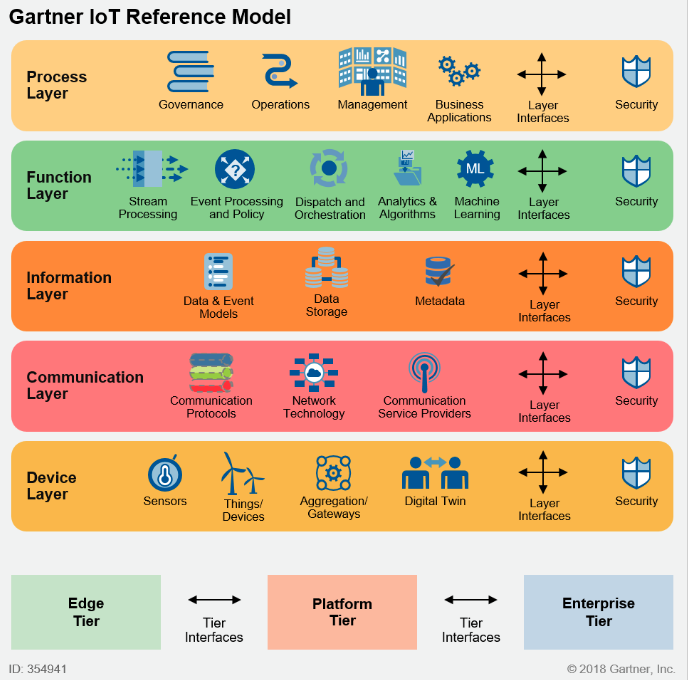
\includegraphics[width=100mm,scale=1]{Figures/gartnerIoT}
	\decoRule
	\caption[Gartner]{Gartner Layer Model}
	\label{fig:gartnerIoT}
\end{figure}



\subsection{Five-Layer architecture}
One by the authors of \parencite{fiveLayer1,fiveLayer} proposed model is a five-layer-model consisting of the following layers.
\begin{description}
    \item [Perception layer] \hfill \\
    The perception layer is the physical layer of the architecture. Sensors and actuators exist in this layer.
    \item [Transport layer] \hfill \\
     The transport layer transports data from the perception layer to the processing layer. Different network protocols can be used
   \item [Processing layer] \hfill \\
   The processing layer stores, analyzes and channels incoming data. It is also known as the middleware layer.
   \item [Application layer] \hfill \\
   The application layer is responsible for delivering user-relevant data to a user.
   \item [Business layer] \hfill \\
   The business layer manages the whole system, e.g. applications, business and profit models.
\end{description}


When talking about IoT-architectures, one should mention the difference between cloud and fog/edge based architectures. 

Cloud based architectures assume that processing and analyzing of data should happen in an enviroment remote from the devices' location.
The network below sends data to the cloud, and above the cloud lie applications working with the processed data with the cloud in the center of this architecture.
In the last years, cloud computing has gained popularity, also in the context of IoT architectures \parencite{CloudComputing} because it provides great exibility and scalability.

A newer trend instead are fog or edge based architectures, where the sensors and gateways do parts of the data processing and analytics.
A fog architecture \parencite{FogComputing1, FogComp} presents a layered approach, inserting various layers between the physical (perception) and transport layers 
(monitoring, pre-processing, storage, security). 
Wheras fog computing refers to smart sensors and gateways, edge computing refers to not-smart objects like motors, pumps with 
smart data preprocessing capabilities \parencite{edgeFog}.


\section{Front-End}
As \parencite{frontendDef} states:
"A front-end system is part of an information system that is directly accessed and interacted with by the user to receive or 
utilize back-end capabilities of the host system. 
It enables users to access and request the features and services of the underlying information system."  

The front-end is the visual component of any application. 

Disciplines like UX (User Experience), UI(User Interface) and  IxD (Interaction design) have been working on creating 
a "better" front-end-experience for many years. 

Usually, a mixture of HTML, CSS and Javascript is used for front-end development. 
In recent years, libaries and frameworks that encourage a component-based architecture are becoming increasingly popular.
The most popular representatives are currently React.js, Angular and Vue \parencite{reactjsAngularVue} 
, where the former two are established tools and the later has been on the rise for the last two years.
The table in Figure \ref{fig:frontEndCompare} displays the differences and similarities between the three tools.

For choosing the right libary or framework, the displayed categories seemed important.
The learning curve would enable the author to use the framwork fast, as there was no prior experience in any framework.
The relative popularity could dertemine the amount of data one would have access to when researching for information on the framework.
"Loved by developers" is an indicator for the long-term ease of use and how more advanced developments would affect especially future developers.
Noteworthy users indicates what kind of traffic a website with the framework can handle and how the websites using these frameworks look like.

\begin{figure}[b]
	\centering
    \includegraphics[width=125mm, scale=1.25]{Figures/CompareFrontend}
	\decoRule
	\caption[Front End Comparison]{Front-End Comparison}
	\label{fig:frontEndCompare}
\end{figure}

\section{Communication}
There are different ways to communicate between the client and the server of a website. 

HTTP (Hypertext Transfer Protocol) is the most popular way to communicate between a client and a server.
It can be used with different languages and frameworks and is usually implemented considering the REpresentational State Transfer (REST) architectural style.
The REST style requires a communication to 
\begin{enumerate}
    \item Seperate the client (visuals) from the server (data storage)
    \item 
    Communication should be "stateless", which means every time the client requests data from the server, 
    it needs to add every information necessary to send the data back to the client. 
    This is comparable to having to send your phone number with every message while chatting,
    so the person on the other end, who has no prior messages from you saved because they are immediately deleted once he or she answers, can text you back.
    You (the client), are the only one who knows the other persons phone number and anytime you want to hear something from them, you have to initiate the conversation.
    \item The incoming data should be cacheable. 
    Messages coming from the server are tagged "cacheable" or "non-cacheable" so the client is given the right to 
    reuse that response data for later or to delete it after usage.
    \item A uniform interface. 
    "REST is defined by four interface constraints: identification of resources; manipulation of resources through representations; self-descriptive messages; and, hypermedia as the engine of application state."
    \parencite{restful}
\end{enumerate}

Due to its stateless nature, a RESTful HTTP approach always needs the client to request data from the server.
There are different techniques to optimize this kind of communication. A Medium article
\parencite{comSummary} explains the differences with a great analogy: waiting for cake to be ready.
Either the client requests cake from the server every possible second (HTTP Short Polling) and asks for the next cake (data) as soon as it gets a response which would look like this in a conversation: 
\textit{ C: "Is the cake ready?" 
C: "Is the cake ready?"
 C: "Is the cake ready?" 
 S: "Yes" 
 C: "Is the next cake ready?"} ,
or the server holds the request open until the cake is ready (HTTP Long Polling) \textit{C: "Is the cake ready?" - pause -  S:"Yes" C:"Is the next cake ready?"}.
A third option is "HTTP Periodic Polling" which requests new data in a set timeframe. 
Essentially, it works like HTTP Short Polling but by increasing the time between the requests, less traffic is produced and the server is relieved.
AJAX \parencite{ajax} is one of the most famous technologies developed to enable periodic polling.
Still, this technique needs a client to request new content instead of listening 
for new information from the server. 
Chat-applications e.g. shouldn't require the user to wait for new messages longer than necessary.
Those services demand a more reactive and immediate communication.
Also, "sending the phone number" meaning the client information with every message creates overhead for every message.

Websockets pursue this task by creating a bilateral environment for clint-server-exchange. 
This way, the client doesn't need to connect again and again, but listens for events once a connection is established.
Now-a-days, most browsers are websocket compatible.
A study in 2013  \parencite{comAJAXvsWeb} discovered that a WebSockets server consumes 50 \% 
less network bandwidth than an AJAX server.
Furthermore, it stated that a WebSockets client consumes memory at constant rate, 
in difference to AJAX which consumes memory at an increasing rate, and that WebSockets can send up to 215.44 \% 
more data samples when consuming the same amount network bandwidth.

The table below compares RESTful HTTP with Websockets. 

\begin{figure}[b]
	\centering
    \includegraphics[width=100mm, scale=1]{Figures/CompareCom}
	\decoRule
	\caption[Communication Comparison]{REST vs Websocket Comparison}
	\label{fig:CompareCom}
\end{figure}

\section{Back-End}

According to the Oxford Dictionary, a back-end is 
"The part of a computer system, piece of software, etc., where data is stored or processed rather 
than the parts that are seen and directly used by the user" \parencite{backendDef}

The back-end can further be separated into the processing and the storing part of the system.
The storing and retrieving of data is usually handled by a database management system (DBMS).
Different frameworks further process the retrieved data and enable middleware functionalities to connect to other services (like the front-end).
Middleware is "software that acts as a bridge between an operating 
system or database 
and applications, especially on a network" \parencite{middlewaredef}. 
The Table in figure \ref{fig:CompareBackend} 
compares the three most popular framework implementations currently used in web development.
The catogries where chosen to match the front-end technologies' categories
except for the "Packages available" and "Performance" category.

Any of these frameworks possess a "package manager" which allows users to download external libaries directly into their project. 
Those libaries are called "packages" and can be uploaded by every developer.
Therefore, only a small percentage of packages are professionally well-designed. 
The goal of a package is first and foremost to ease the development process of an else difficult to implement feature e.g. routing, translation or database-access.
The frameworks also have different starting capabilities, Node.js e.g. relies a lot more on external packages than ASP.Net.
Still, the "Packages available" indicates, additionally to the "Relative Popularity" category, how much community support is available.

The performance category indicates how fast a framework can handle certain requests. 
This is important for scalability of a project. 
In this case, a benchmarking-test was utilized to estimate general performance \parencite{benchmarkNode.NET}.

\begin{figure}[b]
	\centering
    \includegraphics[width=125mm, scale=1.25]{Figures/CompareBackend}
	\decoRule
	\caption[Backend Framework Comparison]{Backend Framework Comparison}
	\label{fig:CompareBackend}
\end{figure}

\subsection{Database}
A database stores the data, whereas a DataBase-Management-System (DBMS) makes the data accessible from elsewhere.
Famous, established examples for DBMS are MySQL and Oracle.
Most DBMS are heavily influenced by the standardised SQL-language which was first introduced in 1970 by Edgar F. Codd in context with the relational model.
An important idea of the relational model is the concept of database normalization, where related records are linked by a key predicate common to all.
Now-a-days, not relational (NoSQL) DBMS like MongoDB gain market share. 
NoSQL DBMS are mainly used for retrieving and save documents with properties unfit for the SQL-scheme with more unorganized relationships (videos, e-mails, social-media posts).
Table \ref{fig:CompareDb} shows different aspects of the 5 most popular DBMS systems.

\begin{figure}[b]
	\centering
    \includegraphics[width=125mm, scale=1.25]{Figures/CompareDb}
	\decoRule
	\caption[DBMS Comparison]{DBMS Comparison}
	\label{fig:CompareDb}
\end{figure}

\section{Device}
%Talk about Arduino implementation
An IoT-Device can take many forms: 
Sensors and actuators can be used to create nearly any use case, 
from motion detection for light automation, to tracking the productivity of a machine to automated heating depending on room temperature.

\subsection{Arduino}
A popular choice for self-made technology projects is the Arduino microprocessor.

Arduino is a microcontroller-company from italy which was founded in 2005. 
It is completely open source and provides its own Integrated Development Enviroment(IDE) \parencite{arduinoIDEDownload}.
The IDE works with nearly all microprocessors on the market. 
The IDE recommends a structure for all Arduino programs:
\begin{description}
    \item [Initialization]
    Prior to any function, libaries and necessary variables are declared within an Arduino program.
    \item [setup()]
    The setup-function is the first function called in any Arduino-program. 
    This is were variables, supporting hardware or the serialport are initialized and pin modes are set. 
    \item [loop()]
    The loop-function loops consecutively, 
    which enables the program to change and respond on run-time.
    Checking for changes usually happens here, 
    whereas consequences of those changes are implemented outside the loop-function.    
\end{description}
The Arduino (and comperable microprocessors) are programmed in C.

Right now, the Arduino is not the most typical choice for IoT-devices in particular as Arduinos 
with included supporting hardware (e.g. Wi-Fi-modules) released just this year,
however due to it's popularity many libaries and instructions exist to introduce an Arduino to an IoT-scope.
E.g. with additional hardware like a Wi-Fi shield and existing free apps like "Blynk"  \parencite{blynk}, 
an Arduino can be tracked and controlled within 30 minutes of set-up.

\section{Summary}
As one can see, a lot of options are available when developing an IoT-project.
Different architectures, protocols, devices, and software settings blow up the decision making process.
Communication protocols and platforms available for other protocols weren't explained in further detail since they were not appliable to the current project settings.
While there is no industry standart, it can be mentioned that a lot of open source and commercial software is developed for different projects.
A good example is "The Things Network" \parencite{ttn} which tries to make IoT accessible for everyone with LoRa-Wan.
This technology needs only a few gateways within a city instead of every user having to build their own gateway.
Even easier to integrate are IoT-devices using the MQTT protocol with e.g. Amazon Web Services \parencite{awsIOT} or the Microsoft Azure Cloud technology \parencite{msIOT}.
For this use case though, an integration platform had to be developed by scratch.

